\clearpage

\section{Práctica 2: Fuente de corriente}



\subsection{Introducción}
La fuente de corriente es un circuito capaz de entregar un cantidad de corriente el cual no depende del valor del voltaje entre la entrada y salida. Aunque en la realidad es necesario colocar una resistencia en paralelo debido a la pérdida del valor ideal.

La simbología de esta fuente es una flecha, y su direción inidica el signo del valor sobre todo el sistema teniendo en cuenta la tierra o común.

La necesidad de desarollar una fuente de corriente es debido a que una señal que es transmitida en variación de corriente tiene mucha presición y con menos ruido que con otra mediante variación de voltaje \parencite{routimo2007comparison}.

\subsection{Marco teórico}
\subsubsection*{Diodo Zener}

\begin{figure}[h]
    \centering
    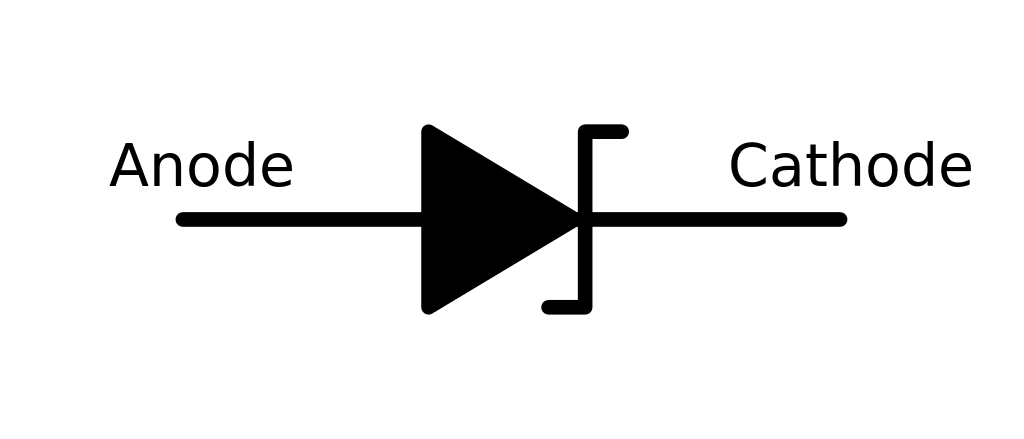
\includegraphics[scale=0.2]{media/1024px-Zener_diode_symbol.svg.png}
    \caption{Simbología del Diodo Zener.}
    \label{Fig: Simbologia del Diodo Zener}
\end{figure}


Es un diodo de silicio fuertemente dopado que es usado para las fuentes de voltaje y corriente debido a sus funciones
diferentes a lo de un diodo rectificador básico. La diferencia está en que, al administrar una alimentación inversa,
el diodo mantendrá una tensión constante. Esto servirá como un regulador de voltaje para la fuente de corriente.

\subsection{Circuito}
Esta práctica consta de dos etapas: el desarrollo de una fuente de corriente constante a 4.4 mA, y otra fuente
 de coriente variable que entregue entre 4 y 20 mA.

A continuación de presentan el primer circuito, fundamento de esta práctica:
\begin{figure}[h]
    \centering
    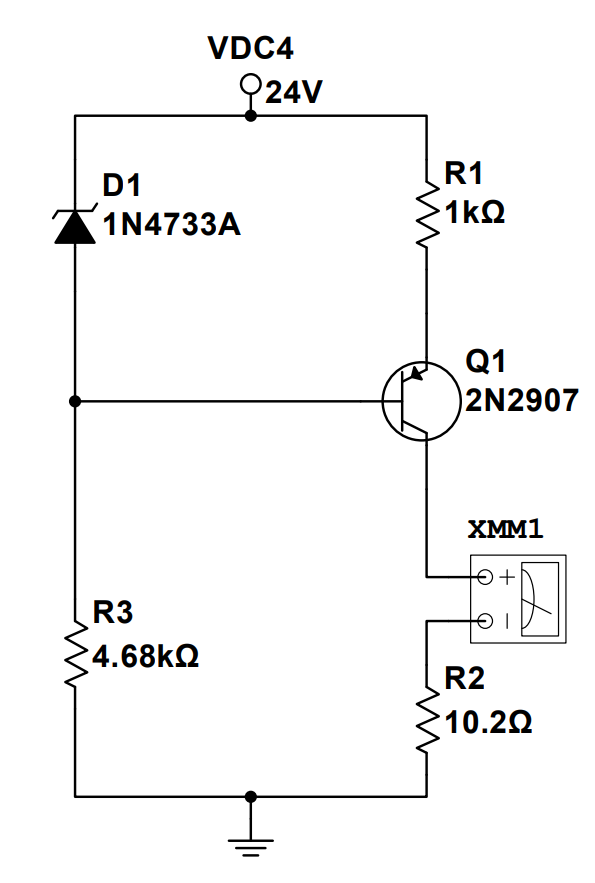
\includegraphics[scale=0.35]{media/Screenshot 2022-05-25 012610.png}
    \caption{Fuente de corriente de 4.4mA}
    \label{Fig: Fuente de corriente de 4.4 mA}
\end{figure}

Como se puede observar, este circuito cuenta con dos etapas, la de generación de corriente, y retroalimentación. La
etapa de generación de corriente consta de un lazo entre el Zener, la base y emisor del transistor y la resisencia de
1k \(\Omega\) . Al igualar a cero el lazo, podremos obtener la corriente de la resistencia y, por ende, de la salida de
la fuente de corriente:
\[ V_R + V_EB - V_Z = 0 \]
\[ i(1k \Omega ) + 0.7V -5.1V = 0 \]
\[ i = \frac{4.4}{R} \]

Al final se obtiene:
\[ i = 4.4 mA \]

La segunda etapa es la salida de la corriente obtenida. Como se puede observar, únicamente contiene dos resistencias, la de
carga (la que contiene el multímetro medidor de corriente) y la de 4.68 k\(\Omega\). La de 4.68k en realidad forma parte de
la etapa de regulacion del diodo Zener porque, juntos, forman un lazo junto con la fuente de 24 V. Esto como consecuencia regula
al mismo tiempo la salida de corriente.

El siguiente circuito no es más que el mismo que el primer caso pero con la capacidad de modificar el valor de corriente de salida.
Para ello, ante tanto valores constantes como el voltaje Zener y el voltaje emisor/base, dentro de la etapa de control se tiene
que volver un valor cambiante la resistencia que antes era de 1 k \(\Omega\). Esto se logra en el arreglo mostrado en la imagen
siguiente (página siguiente).

\begin{figure}[htb]
    \centering
    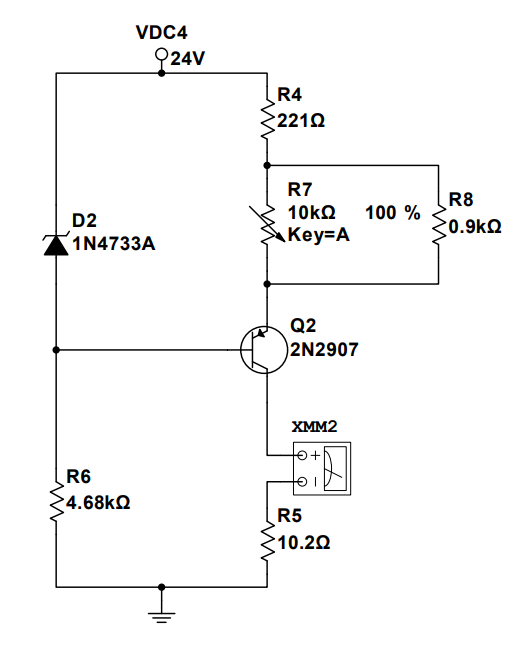
\includegraphics[scale=0.6]{media/casoB.png}
    \caption{Fuente de corriente de 4 a 20 mA}
    \label{Fig: Fuente de corriente de 4 a 20 mA}
\end{figure}

Consta de un arreglo de tres resistencias, dos puestas en paralelo en la que incluye una variable de 10 k\(\Omega\) junto con
otra constante de 0.9 k\(\Omega\). Al calcular la equivalente junto con la de 220 \(\Omega\), el valor de la corriente se obtiene:
\[ R_eq = \frac{4.4}{220 + \frac{900*R_v}{900 + R_v}} \]

Así, la fuente dará el mayor valor de corriente (20 mA esperados) cuando la resistencia variable baje a cero, y el mínimo (4 mA)
cuando ocurra lo contrario.

\subsection{Resultados}

\begin{figure}[htb]
    \centering
    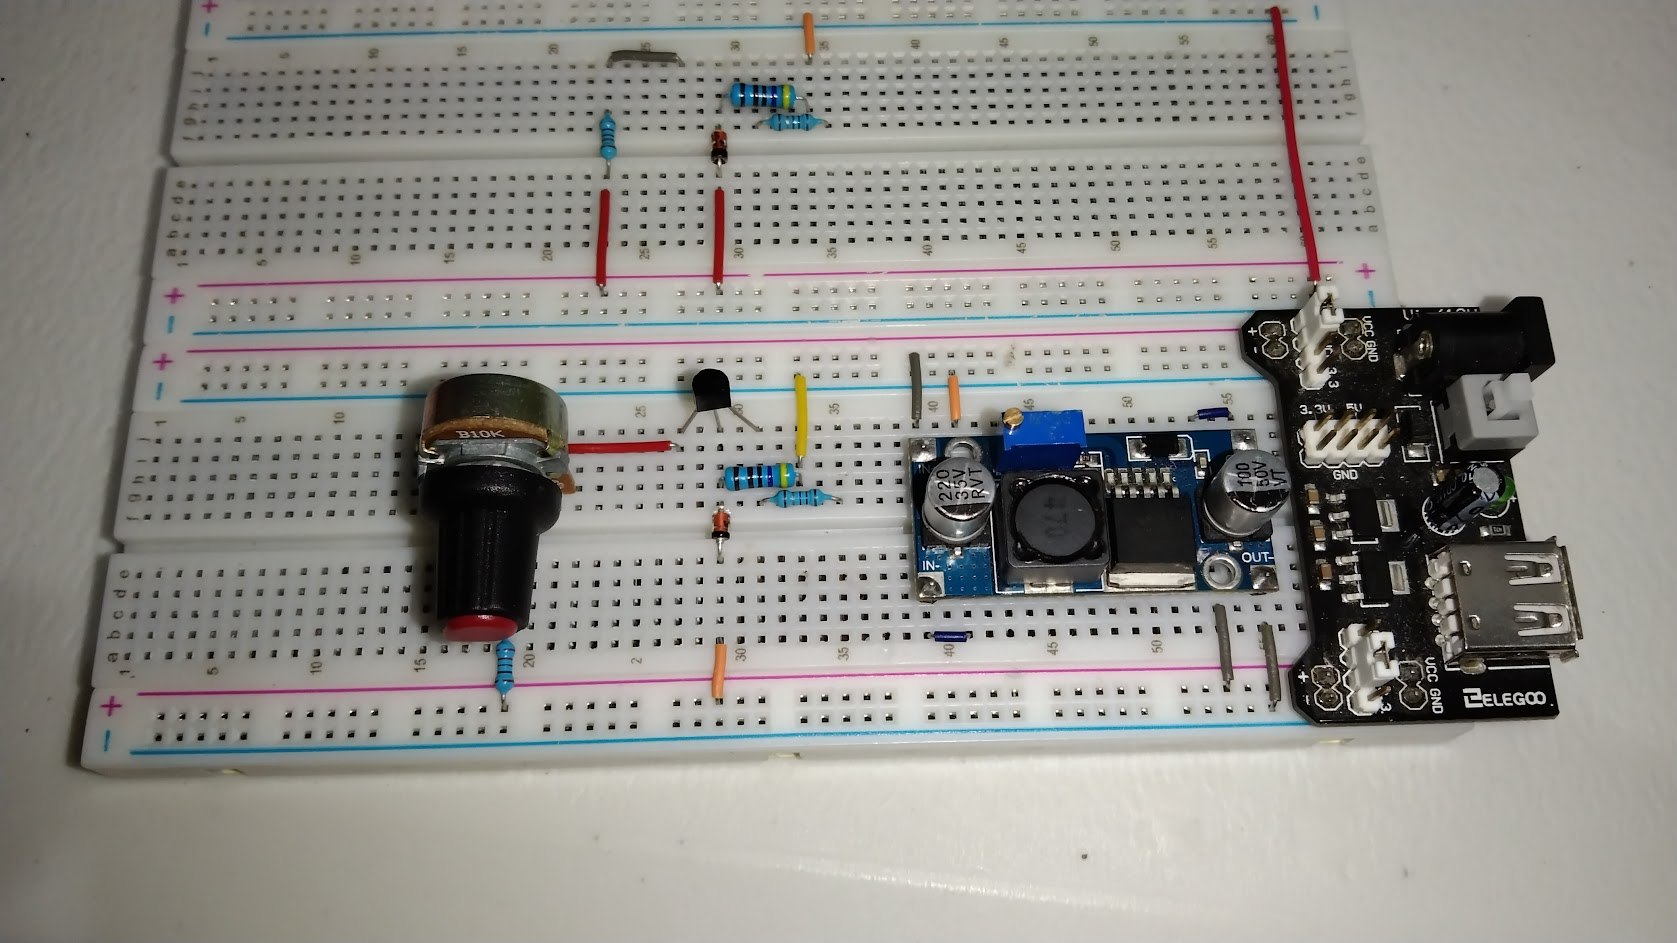
\includegraphics[scale=0.1]{media/IMG_20220303_191602.jpg}
    \caption{Desarrollo de práctica}
    \label{Fig: Desarrollo de práctica 1}
\end{figure}

\begin{figure}[htb]
    \centering
    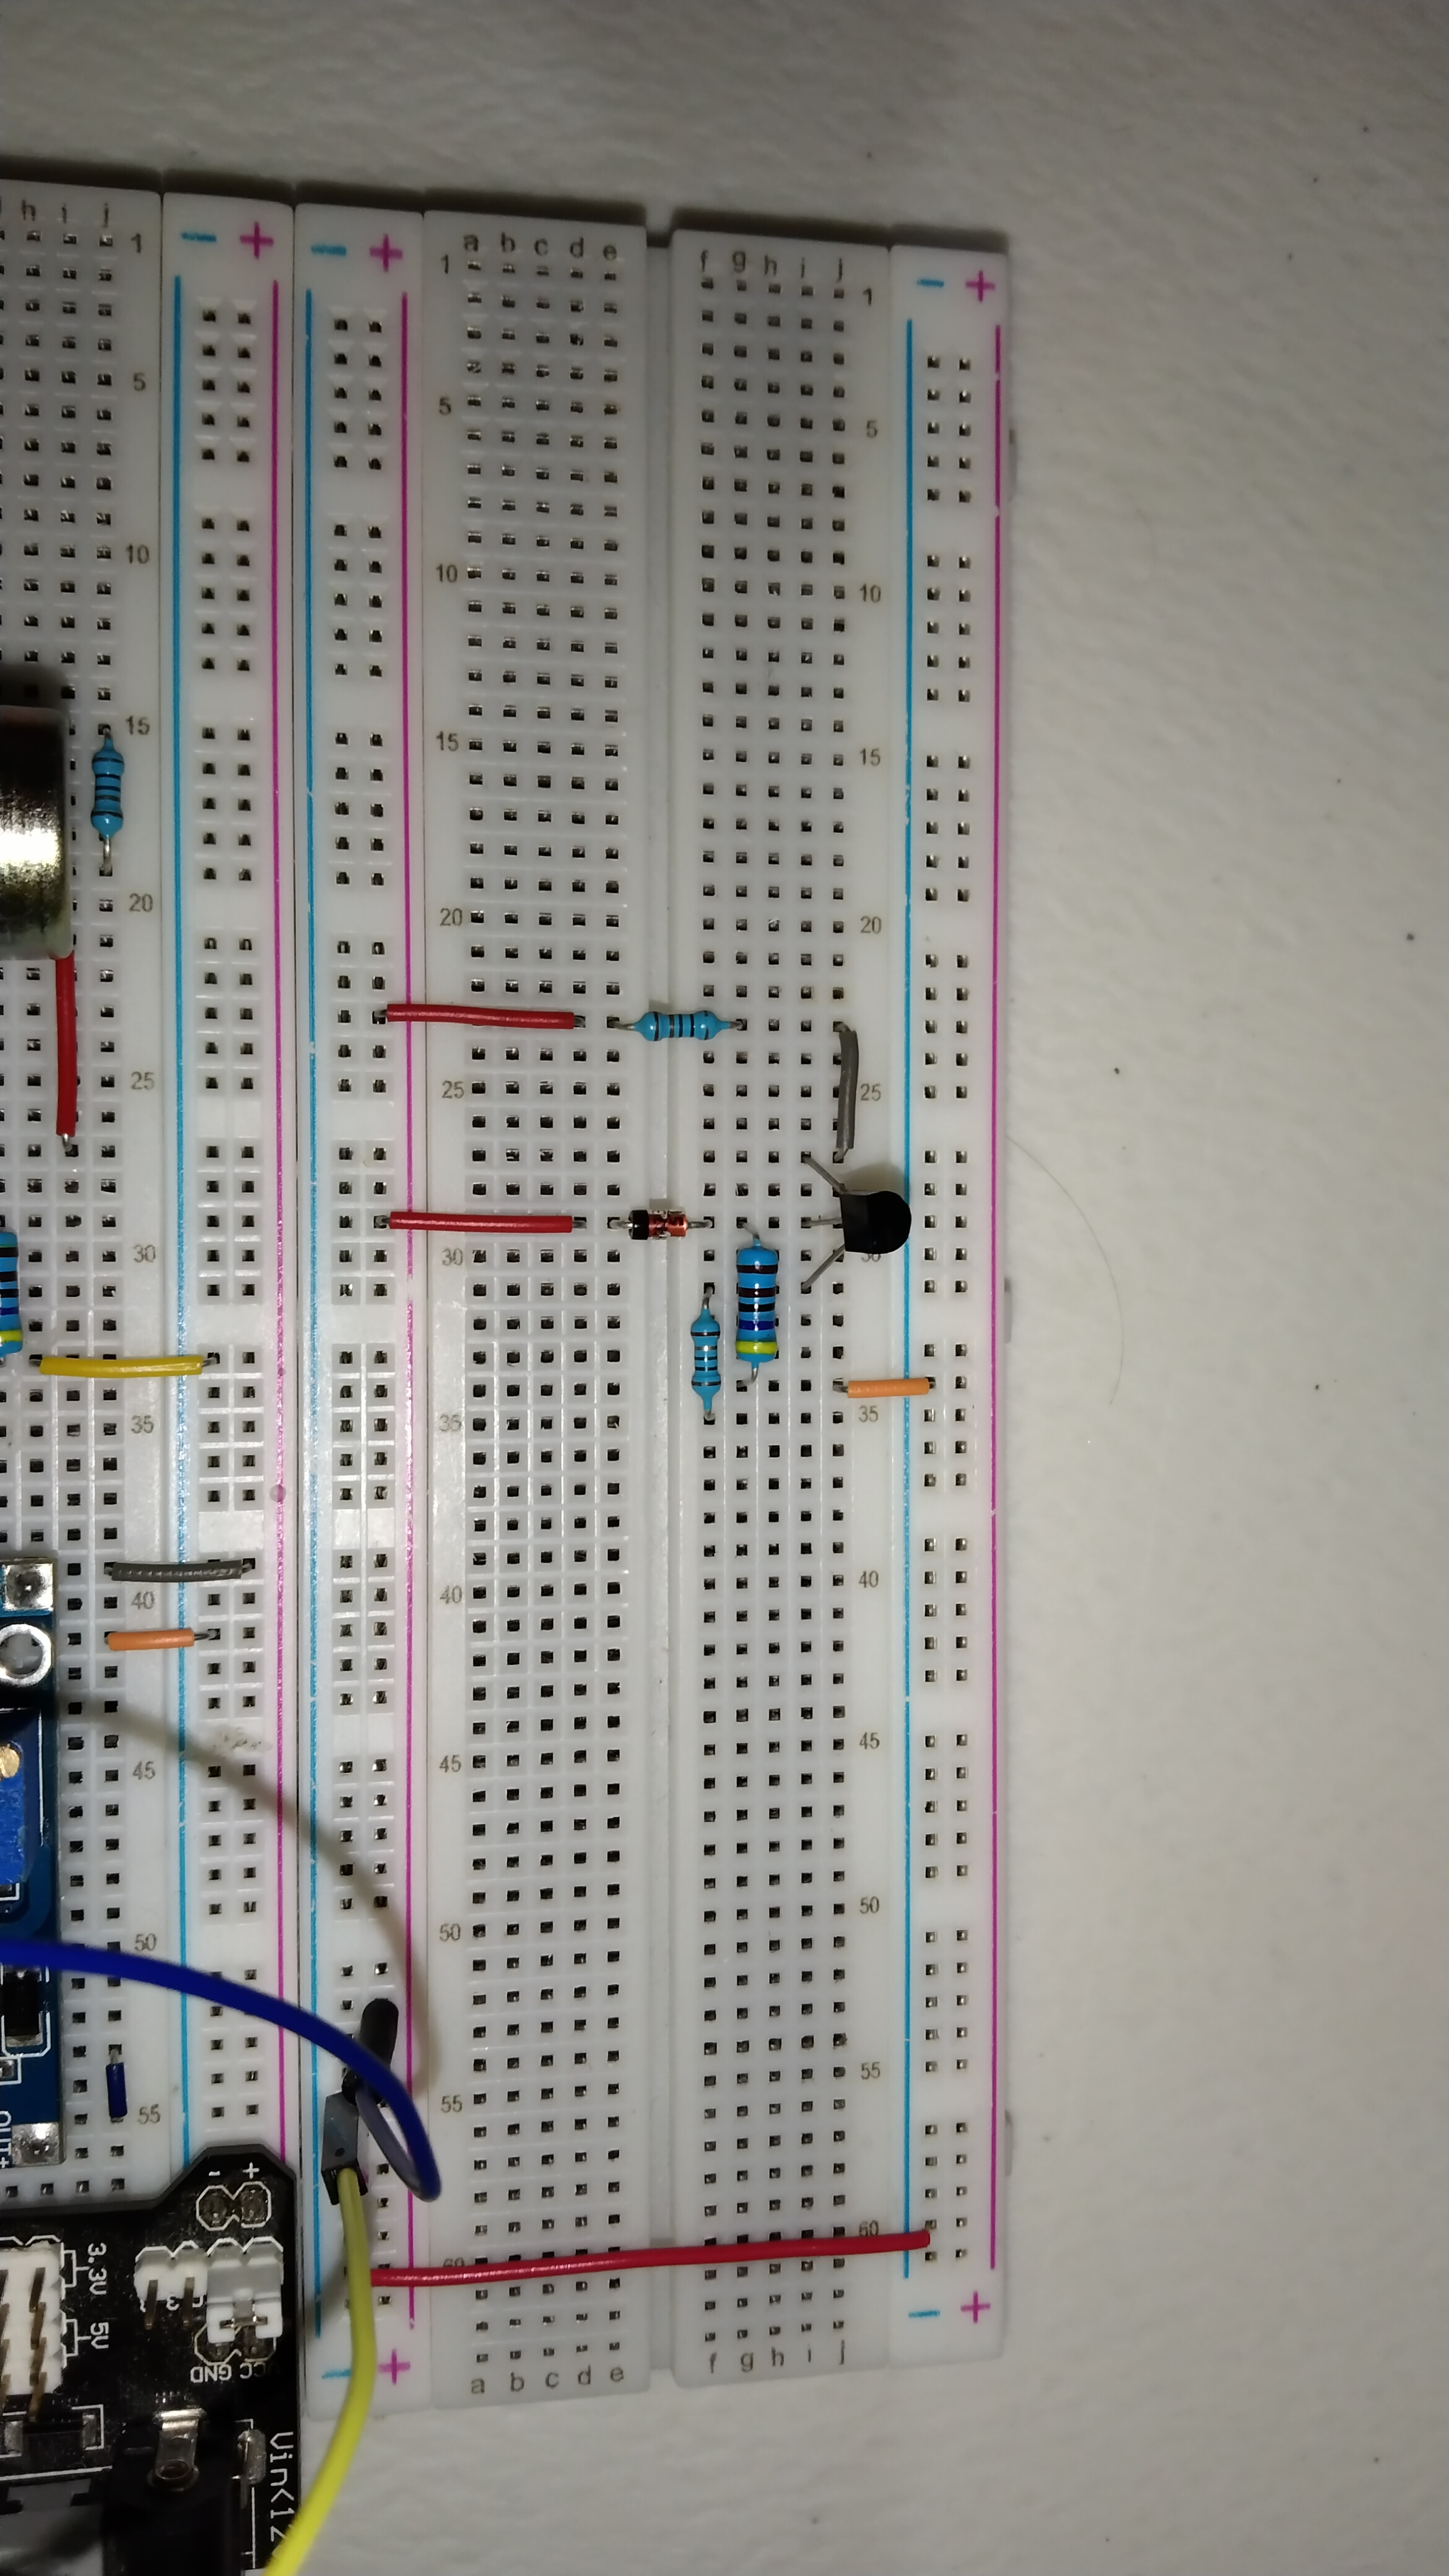
\includegraphics[scale=0.05]{media/imagen2.jpg}
    \caption{Desarrollo de práctica 2}
    \label{Fig: Desarrollo de práctica 2}
\end{figure}

Como se puede obervar, parte de la alimentación de 24 V consta de un alimentador 5V el cual la provee un cargador de teléfono
de 5V a 2A y de un conversor DC-DC tipo elevador, con entrada de 5V y salida a 24V para ambos casos de la práctica. Como
aclaración, se usó el mismo transistor para los dos casos.

El caso A es el que está en el fondo del arreglo de placas de prueba, y el caso B es que tiene el potenciómetro que funciona
como resistencia variable.

Como resultados, para el caso A, se logró obtener una resisencia de 4.4 mA, así como para el caso B el cual es capaz de entregar
corriente con valores de entre 4 y 20 mA.


\subsection{Conclusiones}
La fuente de corriente no es una fuente como tal, si no un arreglo que modifica el potencial de la salida del multímetro
para entregar una corriente constante o una señal de corriente.

Con este arreglo es posible enviar señales eléctricas mediante manipulación de corriente.

Al usar arreglos de resistencias es posible llevar este concepto a los sistemas de comunicación, y de situar el arrglo como
un emisor o receptor de información, usando transductores, puente de Wheatstone para recibir información en sistemas de
intrumentación a nivel industrial.
